\documentclass[10pt]{article}
% We could also do
% \documentclass[10pt, twoside]{article}
% which shifts everything slightly to the
% side which makes it easier to read if
% it's all stapled together. 
\usepackage[doublespacing]{setspace}
\usepackage{mathtools}
\usepackage{array}
\usepackage{booktabs}
\usepackage{float}
\usepackage{amsmath}
\usepackage{amsfonts}
\usepackage{amssymb}
\usepackage{amsthm}
\usepackage{enumitem}
\usepackage{graphicx}
\usepackage{xcolor}
\usepackage{geometry}
\usepackage{titling}
\graphicspath{{.}}
\newtheoremstyle{named}{}{}{}{}{\bfseries}{.}{.5em}{\thmnote{#3}}
\theoremstyle{named}
\newtheorem*{nthm}{Theorem}
\setlength{\droptitle}{-10em}
\title{Optimizing the Robotics Closet}
\author{Sasha Krassovsky, John Lim, Andrey Ryabtsev}
\begin{document}
\maketitle
\begin{abstract}
The present organization of the closet space allocated to the University of Washington's Husky Robotics team leaves much to be improved. With carefully selected simplifying assumptions, we propose a linear programming solution to the closet organization problem. Although the general packing problem is NP-hard, this application allows for a relatively reasonable simplification to one dimensional space with duplicating each shelf to represent multiple layers of items depth-wise and height-wise. The items are optimized for how distant the shelf they are put into is, and futher arranged within each shelf by probability of access. We used the Gurobi python package to solve the MILP problem, and a custom HTML5/JS script to visualize the solution output by Gurobi. The result is an organization scheme that, when implemented, can be expected to improve the average time spent when visiting the closet.
\end{abstract}
\begin{center}
\includegraphics[scale=0.15]{rover.png}
\end{center}
\pagebreak

\section{Introduction}
The Husky Robotics team is a team of both undergraduate and graduate students
from UW building a Mars rover to compete in the University Rover Challenge.
The rover must perform a variety of tasks, such as autonomous navigation, soil
collection, and typing on a keyboard with a robotic arm. The team is divided
into subsystems: Chassis, Arm, Science, Electronics, Software, and Manufacturing.
The subsystems work independently but collaborate to create the robot. Given
all these tasks and the relatively short amount of time given to build out the
functionality, efficiency is key when it comes to the build process.
\par
The robotics team has only a small closet in the Mechanical Engineering Building.
The closet stores the robot along with all of the tools, electronics, sheet metal,
carbon fiber, and plastics that go into building the robot. Each item belongs to
one of the subsystems, and is usually stored near other items belonging to that
subsystem. Unfortunately, the robotics closet is not particularly organized, and
members often spend on the order of 10 minutes looking for the thing they needed.
Our goal is to find a reorganization plan for the items in the closet such that
expected duration of each closet visit is minimized and items belonging to the
same subsystem are in the same connected component on the shelves. By minimizing the time spent in the closet searching for items, and being able to find multiple items they need in a similar place, the team will have more time to spend building the robot each meeting.
\par
The closet has two shelves, one on each side. One side stores items in
uniformly-sized boxes while the other side has several other classes of items,
such as soldering irons, and boxes of various sizes. The rover is stored in
the middle of the room on a big cart. Behind it is the robotic arm and the
science station. In the back are various metallic cylinders, sheet metal,
wood, and rolls of carbon fiber. By examining the frequencies of retrieval
by each team and treating the closet as a grid, we should be able to produce
a better layout of the closet.
\pagebreak
\begin{center}
  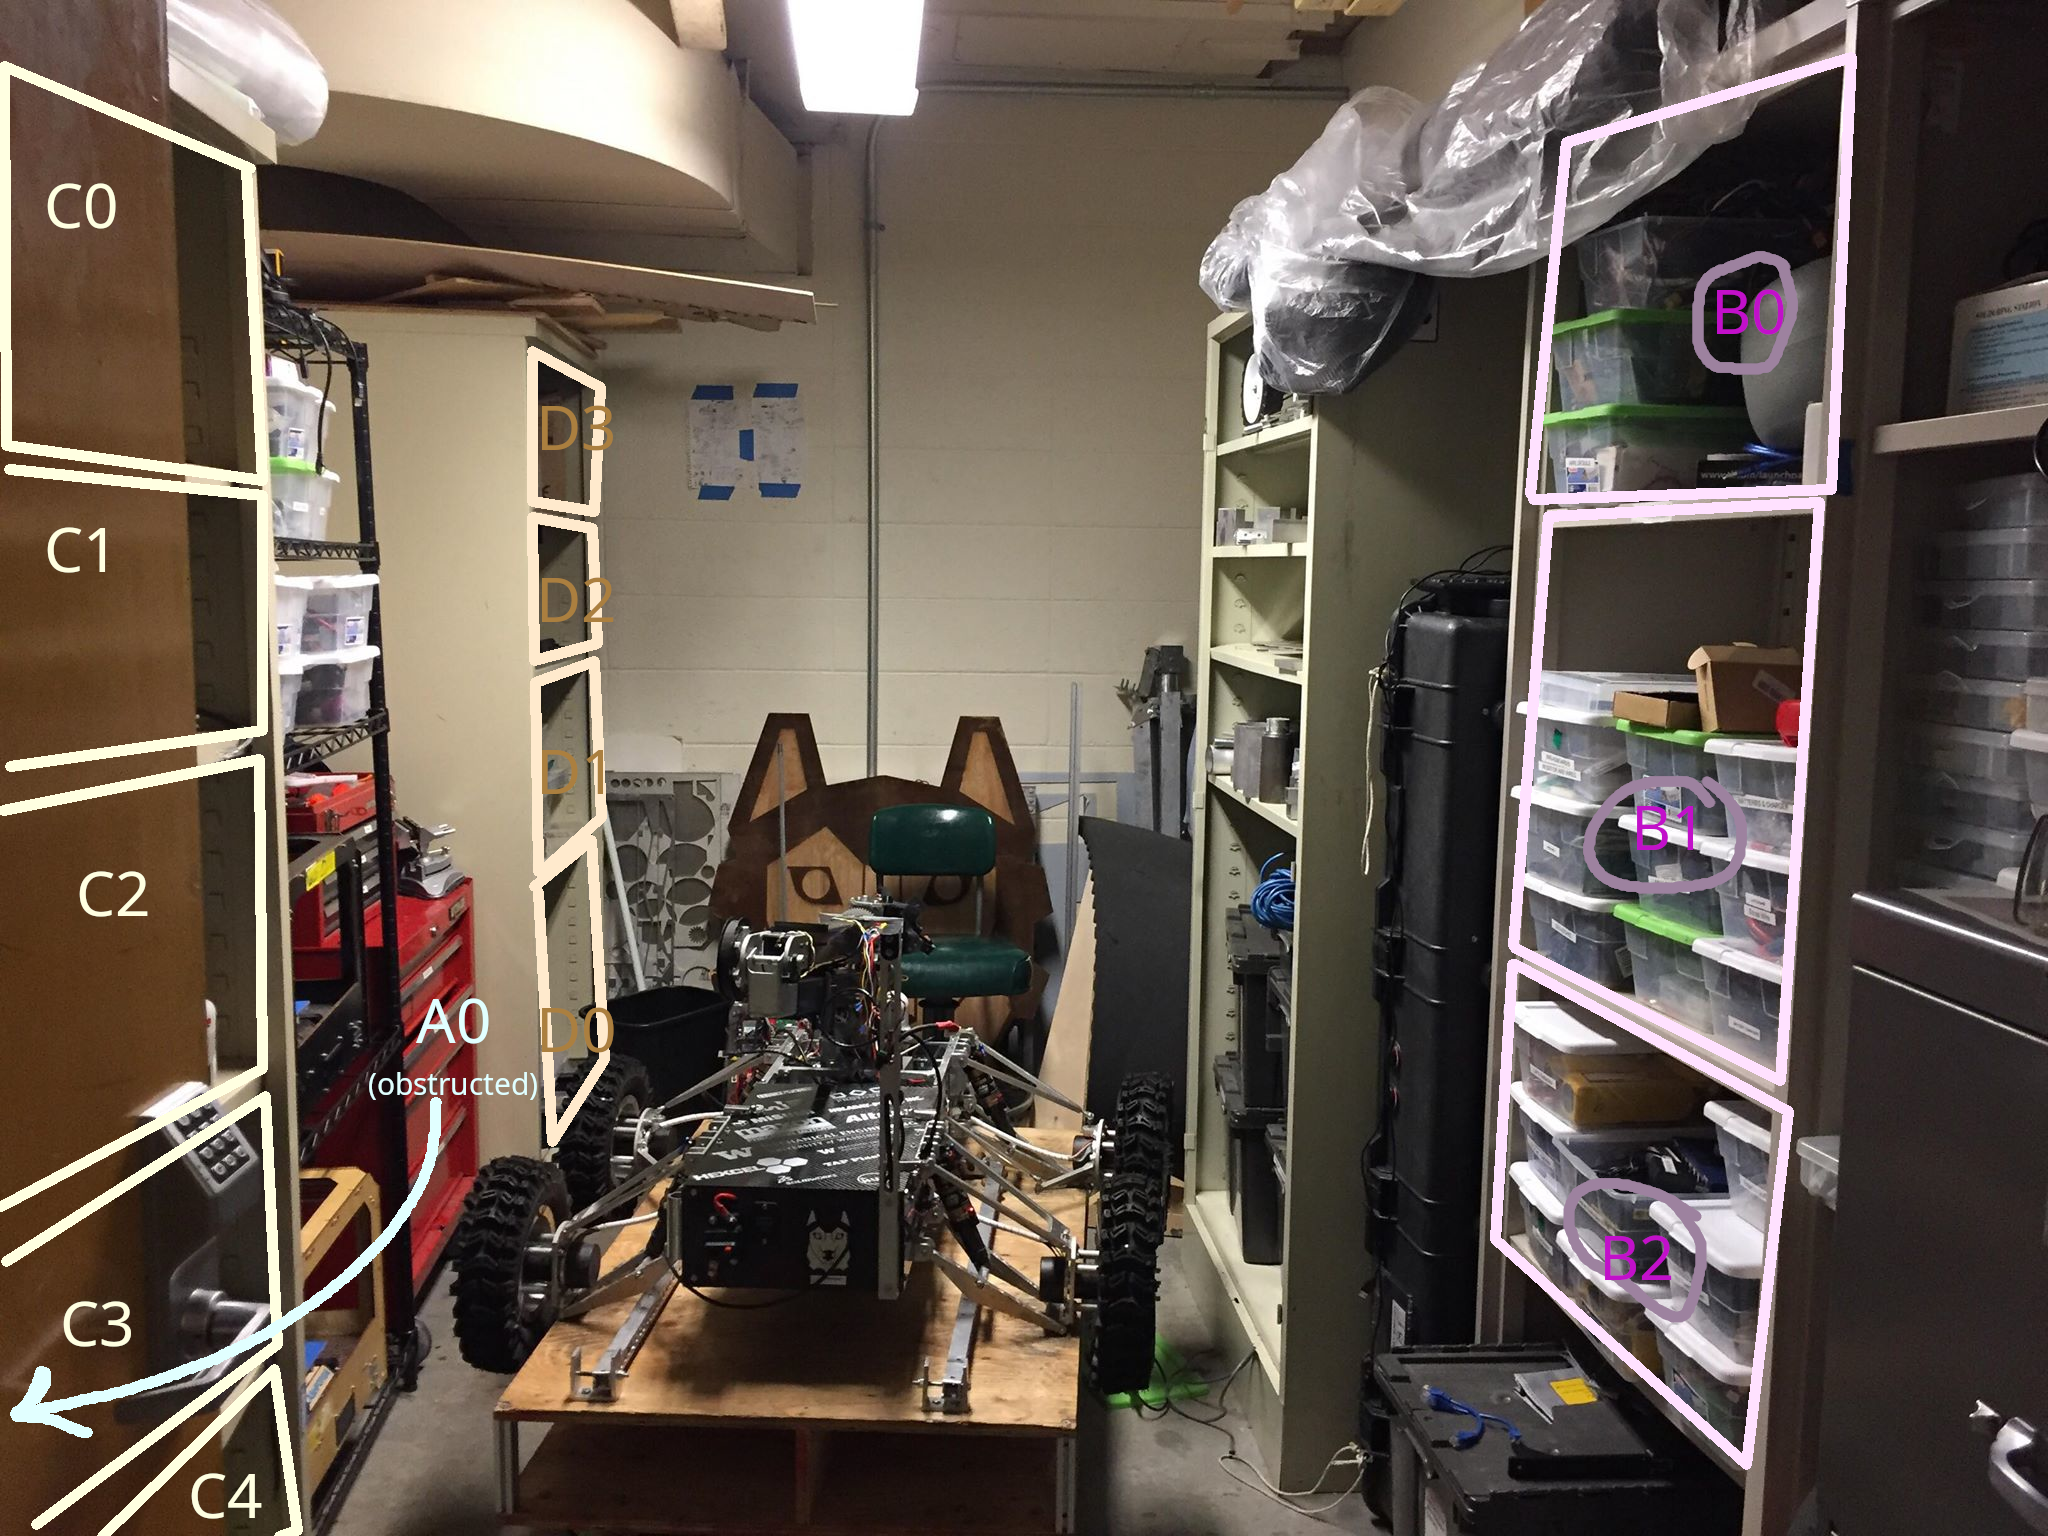
\includegraphics[scale=0.7]{closet2.png} \\
  The robotics closet before optimization. Shelves are labeled to match the solution visualization.
\end{center}

\section{Related Work}
Deepesh Singh's \emph{A Beginner’s guide to Shelf Space Optimization using Linear Programming}
\cite{india} explains an integer programming formulation for finding the optimal layout
of a store that maximizes sales. The guide organizes the store into several racks, each
with a certain number of shelves. One key assumption is that only one product can fit
on a rack. The model uses a table showing how many sales are generated by each item
depending on which rack it is placed. The objective function is then the profit
generated by a given arrangement. Arrangements are represented by a matrix, with
each $a_{ij}$ representing whether product $j$ is on shelf $i$. If it is, the
$a_{ij}$ is $1$ and $0$ otherwise. The guide shows how to maximize this profit function.
Although this approach is a good start, our problem differs in several ways: we can
fit more than one box on each shelf, and our goal is to minimize time of retrieval
rather than maximize profits.

%\textbf{\color{red} TODO: More related work}

\section{Simplifying Assumptions}
\par
Most items in the robotics closet are in boxes. As a result, we assume that all
items are rectangular prisms. Although items such as the chemicals or soldering irons
are not strictly rectangle-shaped, it would be strange for another item reached into
the empty areas of the items' bounding boxes. Taking advantage of this, we approximate
all items as being rectangular prisms, and measure their bounding boxes.
\par
We also assumed that certain parts of the robotics closet are not to be moved. For
example, the shelf containing aluminum brackets and blocks for machining was excluded
from the model entirely. This is due to the cumbersome nature of moving hundreds of
unboxed chunks of metal, and due to opposition to its transportation by team members
who frequently use it. The food pantry portion as well as some non-food items that
made their way into it was similarly excluded after brief deliberation. Excluding
parts of the closet from the model does not reduce the validity of the remaining
optimization since those areas do not intrude on the access to the shelves the model does consider.
\par
We also assumed that there can be on average 3 items in the same 1-D linear
segment. This means that by using some combination of placing items behind
and above other items, we can fit 3 items in that segment. This is a rough
estimate that we came to empirically. This makes sense because some shelves are
very deep, and all shelves fit at least 2 of the boxes vertically, since
the boxes are 12.5 cm tall, and all shelves are taller than 25 cm. 
\par
The previous assumption let us assume for our model is shelves have one unit of depth
and one unit of height. In other words, the model does not have to take into account
insertion of items one behind another. To model height, we make use of the previous
assumption to ``duplicate'' shelves, defining the duplicates to be above the original
one. We can model depth in the same way. 
\section{Model}
We collected data from the robotics closet by measuring each item and shelf. Each
shelf $s$ is represented as an ordered triple $(d, L^{shelf}, c)$, where $d$ is the
distance from the door in ``shelf-lengths'', $L^{shelf}$ is the length of the shelf, and
$c$ is the connected component to which the self belongs.
\par
Each item is represented with an ordered triple $(L^{item}, p, s)$, where $L^{item}$ is the length
of the item, $p$ is the probability that the item is selected, and $s$ is the item's
subsystem. Notice that we represent each item as a 1-dimensional length. This is valid
because we assumed that each shelf had a single unit of depth and a single
unit of height. As a pre-processing step, minimize the length. Since we cannot always
rotate an item into a horizontal orientation, for an item with dimensions $a \times b$
the item's 1-dimensional length is given by 
$$L^{item} = \min(a, b)$$
\par
Let there be $n_0$ shelves and $m$ items, $k$ subsystems, and $n_c$ be the number of
connected components. In order to simulate stacking and placing behind, we
multiply the number of shelves by our assumed average number of items per
1-dimensional block. In our model, we chose 3 as our constant. Thus,
the total number of shelves in the model is $n = 3n_0$. 
Our decision variables lie in two matrices
$$W = (w_{ij}), 1 \leq i \leq n, 1 \leq j \leq m$$
$$C = (c_{ij}), 1 \leq i \leq l, 1 \leq j \leq k$$
Each $w_{ij}$ and $c_{ij}$ is a binary variable, i.e. each $w_{ij}, c_{ij} \in {0, 1}$.
Each $w_{ij}$ is $0$ if item $j$ is not on shelf $i$ and $1$ otherwise. $c_{ij}$ is
$1$ if subsystem $j$ lies in connected component $i$ and $0$ otherwise. 
$C$ is a $n_c \times k$ matrix because there are l connected components and k subsystems. 
Note about notation: ($l^i_k$ indicates the length of item $k$ while $l^s_k$ indicates the
length of shelf k. $I$ is the set of items and $S$ is the set of shelves. For any item
$x$, $p_x$ and $s_x$ represent the item's probability and subsystem respectively. Let
there be $n_0$ shelves and $m$ items, $k$ subsystems, and $n_c$ be the number of 
connected components.)
\par
The model is subject to the following constraints:
\begin{enumerate}
\item $\sum_{j = 1}^{m}w_{ij} L^{item}_j \leq L^{shelf}_i, $ for every $1 \leq i \leq n_0$ ($n_0 = $ number of shelves).
\item $\sum_{i = 1}^{n}w_{ij} = 1, $ for every $1 \leq j \leq m$ ($m = $ number of items).
\item $\sum_{j = 1}^{l}c_{ji} = 1, $ for every $1 \leq i \leq k$.
\item Let $K$ be the set of indices of items belonging to subsystem $i$. Let
  Let $L$ be the set of indices of shelves belonging to connected component $j$.
  Then $\sum_{a \in K}\sum_{b \in L}w_{ba} = |K| \cdot c_{ji}, 1 \leq i \leq k, 1 \leq j \leq l$.
\end{enumerate}
Since each probability $p$ is less than 1, we incentivize putting items with higher probability
in the front by multiplying the probability by the distance. Thus, our objective function
becomes
$$\min z = \sum_{i = 1}^{n}\sum_{j = 1}^{m} d_j p_i w_{ij}$$

\textbf{Explanation of Constraints:}
\begin{enumerate}
\item The sum the lengths of all of the items on a given shelf must be less than or equal to
  the maximum length that the shelf can support. We multiply by $w_{ji}$ so that
  items not included on the shelf are not counted.
\item Each column of $W$ can only have one $1$, because we cannot put an item
  on two shelves simultaneously. Since each row represents a shelf, we simply
  traverse the whole column and ensure its sum is exactly $1$. Notice that if
  we had put $\leq 1$, the constraint would be invalid because then
  no items could have been included. Thus, this constraint implicitly enforces
  the constraint that every item be included.
\item Each column of $C$ can only have one $1$ because all items belonging to
  a subsystem must be in the same connected component, and therefore a subsystem
  can be in exactly one connected component. Similarly to constraint 2, summing
  the column and ensuring that the sum is 1 enforces the idea that every subsystem is
  included.
\item The intuition behind this constraint is that either all items belonging
  to a subsystem are in a given connected component, or none are. Thus, we
  use the decision variable $c_{ji}$ to choose whether the sum is $0$ or not. 
\end{enumerate}

\section{Solution and Results}
We used the Gurobi optimization library to solve the formulated integer programming
problem. The results placed 11 items into Shelf 5, 16 items into Shelf 6, 13 items
into Shelf 7, 13 items into Shelf 8, 11 items into Shelf 9, 2 into 10, 1 into 11,
2 into 12, and 11 into 13. The remaining shelves had no items placed in them.
This confirmed our intuition that there was plenty of space for the items
even with the single depth layer constraint. A brief examination of the items
allocated to each specific shelf provides support for validity of the model;
it is not difficult to imagine the items listed placed compactly, but plausibly.
\par
Only the shelves that have distance 2 (highest distance in the input data set)
are left empty. This is an indication that proximity is, in fact, taken into
account by the model. Finally, LiPo batteries are placed onto the same drawer,
as are NVIDIA Jetsons and other closely related items. This validates that the
connected components constraint is being considered.

\section{Improvements}
We noticed that the model packed together very many items while leaving four
perfectly good shelves empty. Especially when considering that there are items
we likely forgot to catalogue, as well as items that would get added later on,
we may consider adding space remaining in shelves as a soft constraint. This
could be done by either reducing the width of each shelf or by padding the
items on all sides to imply that there must be room between each item. This
would also have the added benefit of making items easier to take out, since
it is illogical to stuff some shelves to the last inch while leaving whole
drawers to collect dust. Unfortunately, the difficulty of making the model work correctly with the 1D simplification presently prevented us from tackling it, but with more time to invest, this could be fine tuned, or the model could be switched to 2D or 3D.

\section{Conclusions}
In conclusion, we are happy to have found an integer programming approach
with the aforementioned constraints and objective function to be successful
at finding a reasonably optimal arrangement of items. We were able to learn
the practical challenges of solving a real-world linear programming problem,
whilst still getting a result that has legitemate applications. 

\section{Acknowledgements}
We would like to thank:
\begin{itemize}
\item Prof. Sara Billey for providing us with guidance throughout the project,
\item Hongyu Cao for supplying us with a paper that inspired a significant portion of our thoughts on the problem,
\item Husky Robotics for providing the closet to undergo optimization,
\item Nolan Donovan for working with us to understand and solve this problem.
\end{itemize}

\section{References}
\begin{thebibliography}{9}
\bibitem{volleyball} Guido Cocchi, Alessandro Galligari, Federica Picca Nicolino,
  Veronica Piccialli, Fabio Schoen, Marco Sciandrone.
  “Scheduling the Italian National Volleyball Tournament.” Interfaces 48(3):271-284, 2018. 
\bibitem{india} Singh, Deepesh. “A Beginner’s guide to Shelf Space Optimization using
  Linear Programming.” Analytics Vidhya, 2016
\bibitem{knapsack} Andrea Lodi, Michele Monaci. “Integer Linear Programming Models for
  2-staged Two-Dimensional Knapsack Problems.” Dipartimento di Elettronica,
  Informatica e Sistemistica, University of Bologna, 2001
\bibitem{imnotamonkeyimascientist} Winston, Wayne. “Operations research:
  Applications and algorithms.” Belmont, CA: Thomson/Brooks/Cole, 2004
\bibitem{siggraph}  Yu, Lap-Fai, et al. “Make It Home.” ACM SIGGRAPH 2011 Papers
  on - SIGGRAPH 11, 2011, doi:10.1145/1964921.1964981.  
\end{thebibliography}
Source code can be found at: https://github.com/save-buffer/math381

\pagebreak
\newgeometry{left=3cm,right=3cm,top=3cm,bottom=3cm}
\section{Appendix: Solution Visualization}
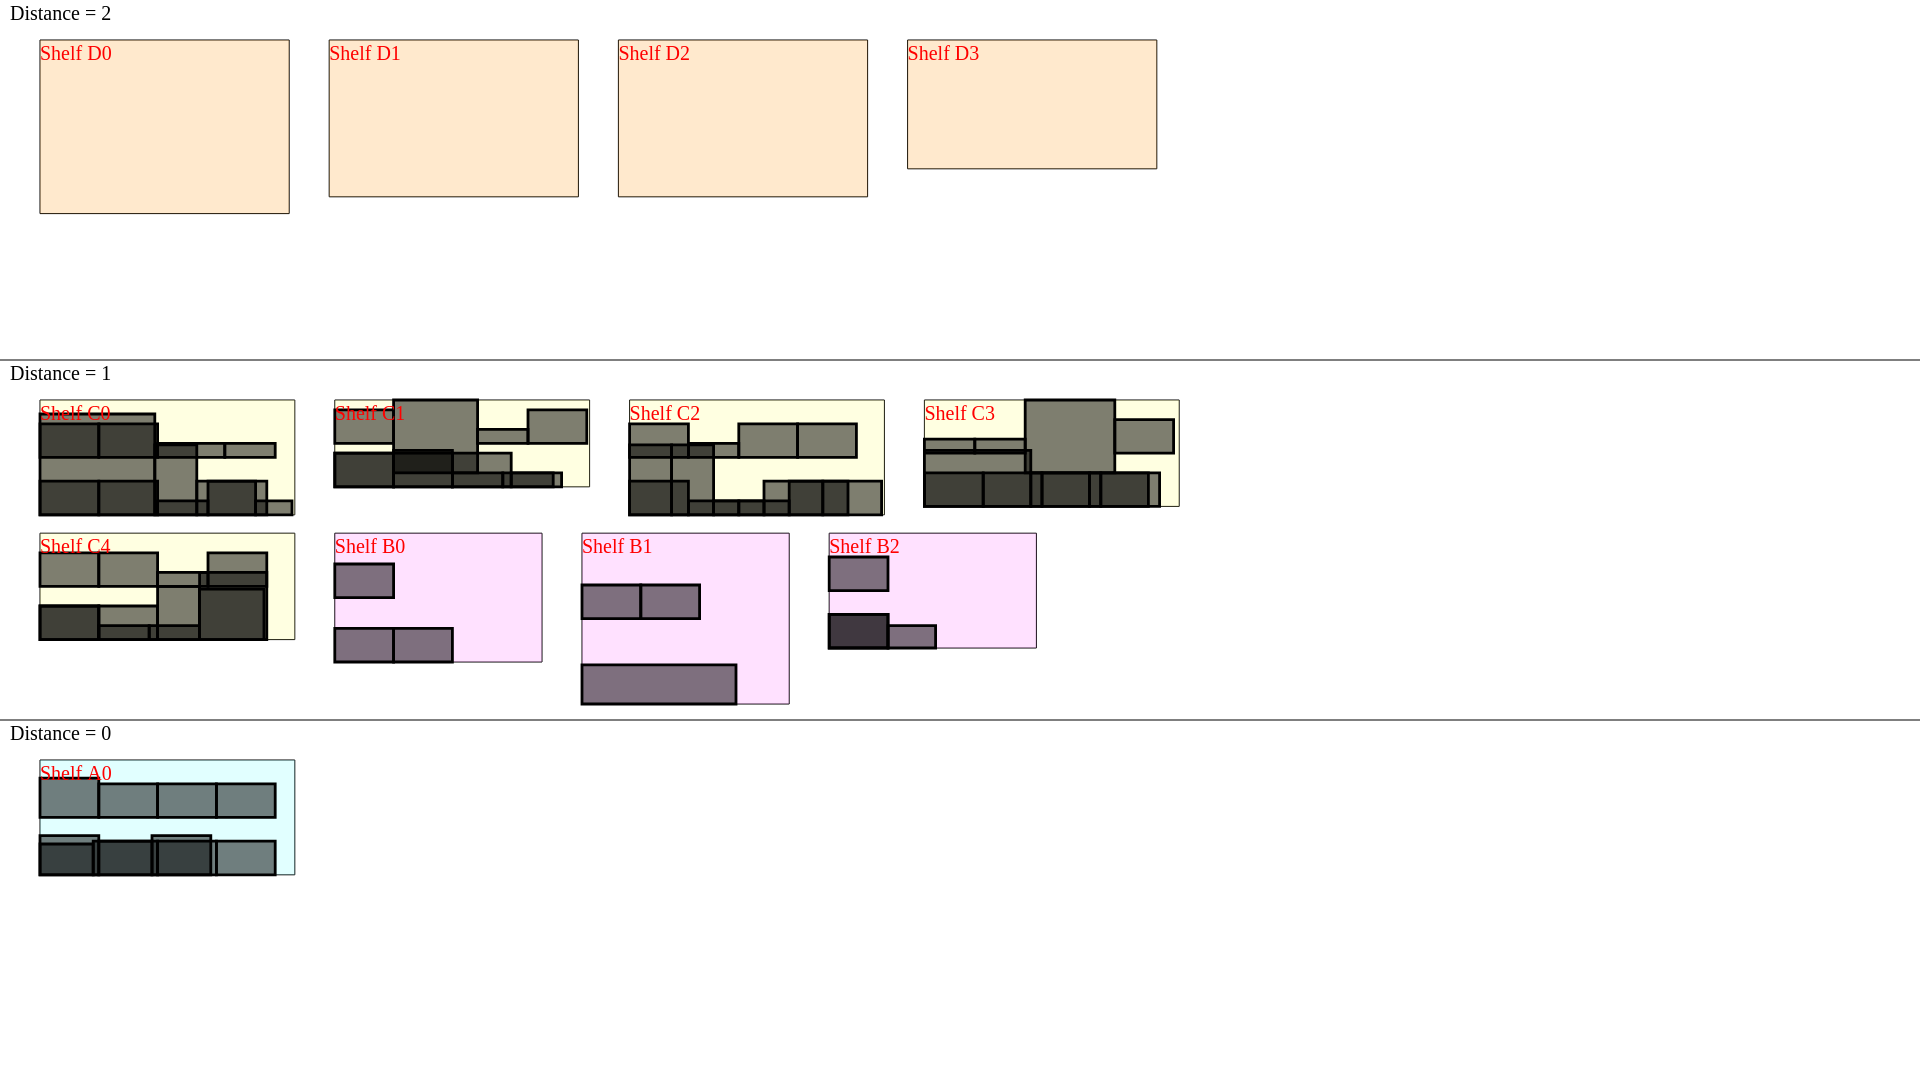
\includegraphics[scale=0.40,angle=90]{image.png}
\end{document}
